\subsection*{Overview}
For the fourth experiment undertaken, it was decided to take inspiration from
\textcite{yanaiFood}, where pre-training was used training a model for food
classification. In order to achieve this, the final layer of the
Inception V3 model which was trained on the ImageNet dataset had to be retrained. This is called
Transfer Learning. A tutorial, created by Google, on the tensorflow website was followed
for direction on this process \textcite{retrainInception}.

Firstly, in order to retrain the final layer of a model, a dataset must be
prepared in the correct way. The Food-101 dataset \textcite{food101}
was used for this experiment, which will be analysed below. The dataset must be structured so that
there is a separated directory for each class with the directory name as the class
name. These directories should contain all the images for this class. 

Once this dataset has been set up correctly, a directory can be found on github
which contains the necessary files for this tutorial. When the directory has
been downloaded, the following command can be ran:
\begin{lstlisting}
python tensorflow/examples/image_retraining/retrain.py \ --image_dir
~/dataset_directory
\end{lstlisting}

The first thing that the script will do is create bottleneck files for the
images. A bottleneck is a term used to define the final layer before the output
layer. This is so that for each image, we do not have to push it through the
entire network during training \textcite{retrainInception}.

After, the bottlenecks are created, the training can be completed. The images
are split into three sub directories of training, testing and validation. By
default, these images are split into percentages of 80\%, 10\% and 10\%
respectively. The model is trained at a default of 4000 steps. 

At the final stage of the script, the model is run on a batch of test images not
yet seen and a final test accuracy is displayed. This can be seen in the Script
section below.

The command used for using this model once it is trained is:
\begin{lstlisting}
python tensorflow/examples/label_image.py --graph=/tmp/output_graph.pb
--labels=/tmp/output_labels.txt --input_layer=Mul --output_layer=final_result
--input_mean=128 --input_std=128 --image=~/image_directory
\end{lstlisting}

\subsection*{Network Architecture}
The Inception V3 model network architecture was used for this experiment. The
Inception V3 architecture was created by building on the existing Inception
model aimed at efficient image classification \textcite{rethinkingInception}.
This research was carried out due to the popularity of convolutional neural networks.
The main aim of this study was to produce a model that would "scale up networks in ways that aim at utilizing the added computation as efficiently as possible by suitable factorized convolutions and aggressive regularization" \textcite{rethinkingInception}.
The team did not want to simply rely on larger models for better results.

The are 4 main design principles that the research team followed in the paper \textcite{rethinkingInception}:
\begin{itemize}
    \item{Avoid representational bottlenecks}
    \item{It is easier to process higher dimensional representations locally}
    \item{Without much loss in power, spatial aggregation can be carried out over lower dimensional embeddings}
    \item{The width and depth of the network should be balanced and when one is increased it can be beneficial to increase the other.}
\end{itemize}

\begin{figure}
     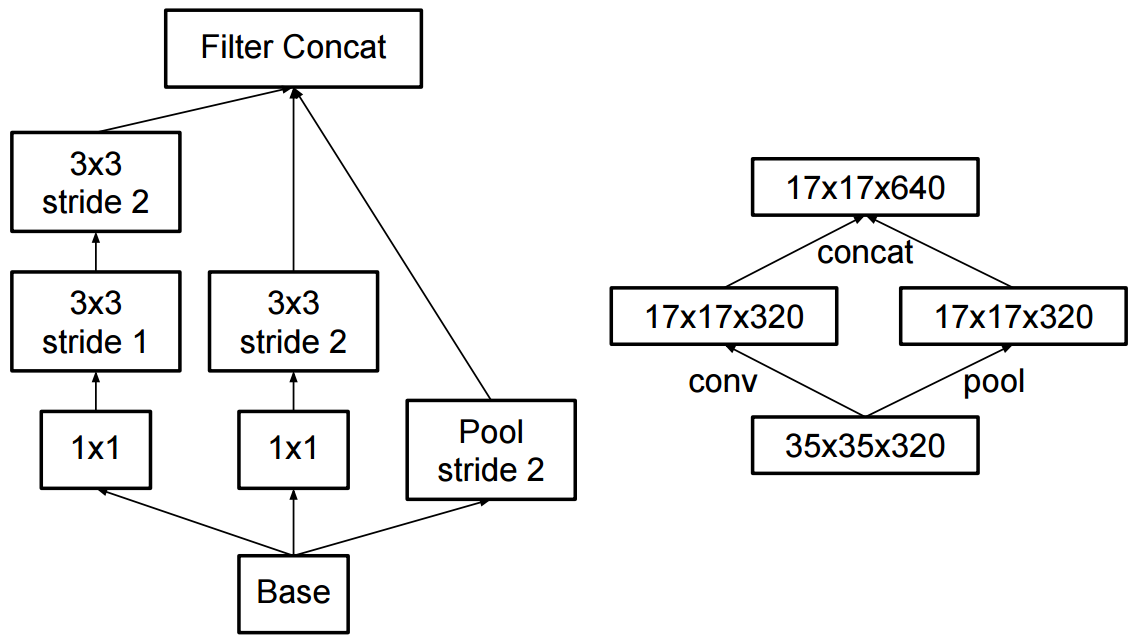
\includegraphics[scale=0.25]{inception}
     \caption{Inception module}
     \label{fig:inception}
\end{figure}

The main idea behind the network is that different strands of the network are followed and the best result is used as seen in Figure \ref{fig:inception}.

In order to combat the problem of low resolution input, three separate experiments were carried out based on the fact that "One simple way to ensure constant effort effort is to reduce the strides of the first two layer in the case of lower resolution input, or by simply removing the first pooling layer of the network" \textcite{rethinkingInception}.

These experiments are as follows, with the first resulting in the most accurate:
\begin{itemize}
    \item{"299 x 299 receptive field with stride 2 and maximum pooling after the first layer." \textcite{rethinkingInception}}
    \item{"151 x 151 receptive field with stride 1 and maximum pooling after the first layer." \textcite{rethinkingInception}}
    \item{"79 x 79 receptive field with stride 1 and without pooling after the first layer." \textcite{rethinkingInception}}
\end{itemize}

\begin{figure}
     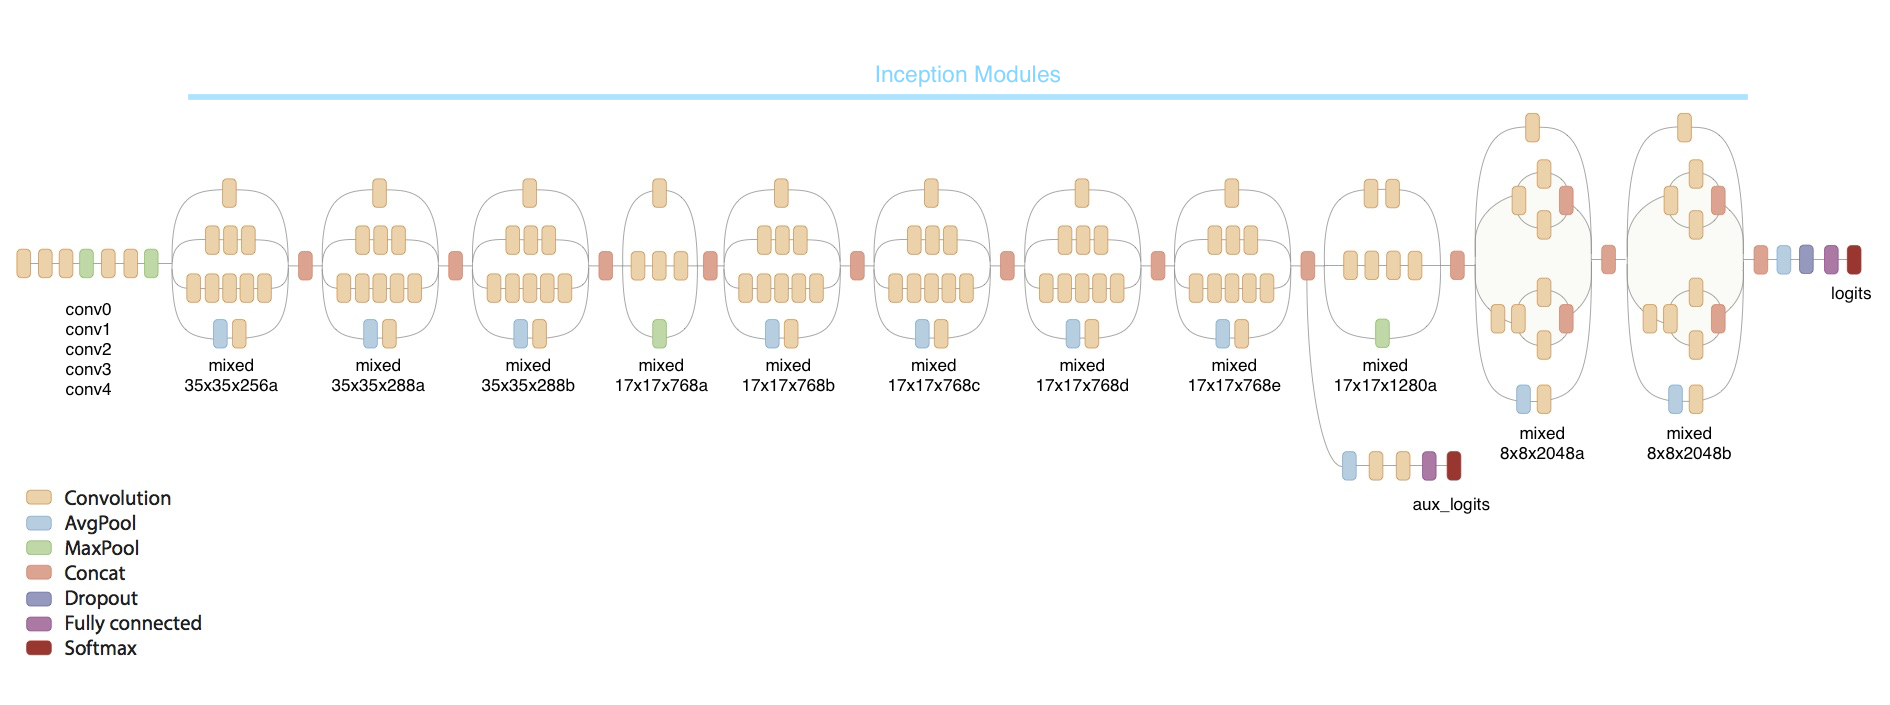
\includegraphics[scale=0.25]{inception_model}
     \caption{Inception V3 Architecture}
     \label{fig:inception_model}
\end{figure}

The best results of the Inception-V3 model achieved 78.8\% top-1 accuracy and 94.4\% top accuracy of the ILSVR 2012 dataset \textcite{rethinkingInception}.
This model also was the least computationally expensive of other published and successful models.
The full model can be viewed in Figure \ref{fig:inception_model}.

\subsection*{Dataset}
The dataset used for this experiment is the Food-101 dataset \textcite{food
101}. This dataset has 101 classes with 1000 images for each class.

\subsection*{Libraries}
Tensorflow and Numpy were used to run this scipt.

\subsection*{Script}
The following snippets of code are from the retrain.py script.

\begin{lstlisting}
# Add the new layer that we'll be training.
(train_step, cross_entropy, bottleneck_input, ground_truth_input,
final_tensor) = add_final_training_ops(
            len(image_lists.keys()), FLAGS.final_tensor_name,
            bottleneck_tensor,
            model_info['bottleneck_tensor_size'],
            model_info['quantize_layer'])
 
# Create the operations we need to evaluate the accuracy of our new layer.
evaluation_step, prediction = add_evaluation_step(
final_tensor, ground_truth_input)
 
# Merge all the summaries and write them out to the summaries_dir
merged = tf.summary.merge_all()
train_writer = tf.summary.FileWriter(FLAGS.summaries_dir + '/train',
                                     sess.graph)
 
validation_writer = tf.summary.FileWriter(
    FLAGS.summaries_dir + '/validation')
 
# Set up all our weights to their initial default values.
init = tf.global_variables_initializer()
sess.run(init)

\end{lstlisting}




\begin{lstlisting}
# We've completed all our training, so run a final test evaluation on
# some new images we haven't used before.
test_bottlenecks, test_ground_truth, test_filenames = (
    get_random_cached_bottlenecks(
        sess, image_lists, FLAGS.test_batch_size, 'testing',
        FLAGS.bottleneck_dir, FLAGS.image_dir, jpeg_data_tensor,
        decoded_image_tensor, resized_image_tensor, bottleneck_tensor,
        FLAGS.architecture))
test_accuracy, predictions = sess.run(
   [evaluation_step, prediction],
   feed_dict={bottleneck_input: test_bottlenecks,
        ground_truth_input: test_ground_truth})
tf.logging.info('Final test accuracy = %.1f%% (N=%d)' %
                (test_accuracy * 100, len(test_bottlenecks)))
\end{lstlisting}

\subsection*{Results}
The final test accuracy for this retrained model was 54.8\%.

For example, an image of pizza Figure\ref{fig:pizza}, was fed into the model with the followng results:
\begin{itemize}
    \item{pizza 0.925}
    \item{pancakes 0.008}
    \item{nachos 0.007}
    \item{beef carpaccio 0.006}
    \item{tiramisu 0.004}
\end{itemize}

\begin{figure}
     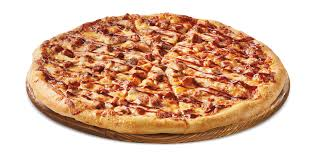
\includegraphics{pizza}
     \caption{Pizza}
     \label{fig:pizza}
\end{figure}

In contrast, Figure \ref{fig:pizza_unclassified} was not classified as a pizza.

\begin{figure}
     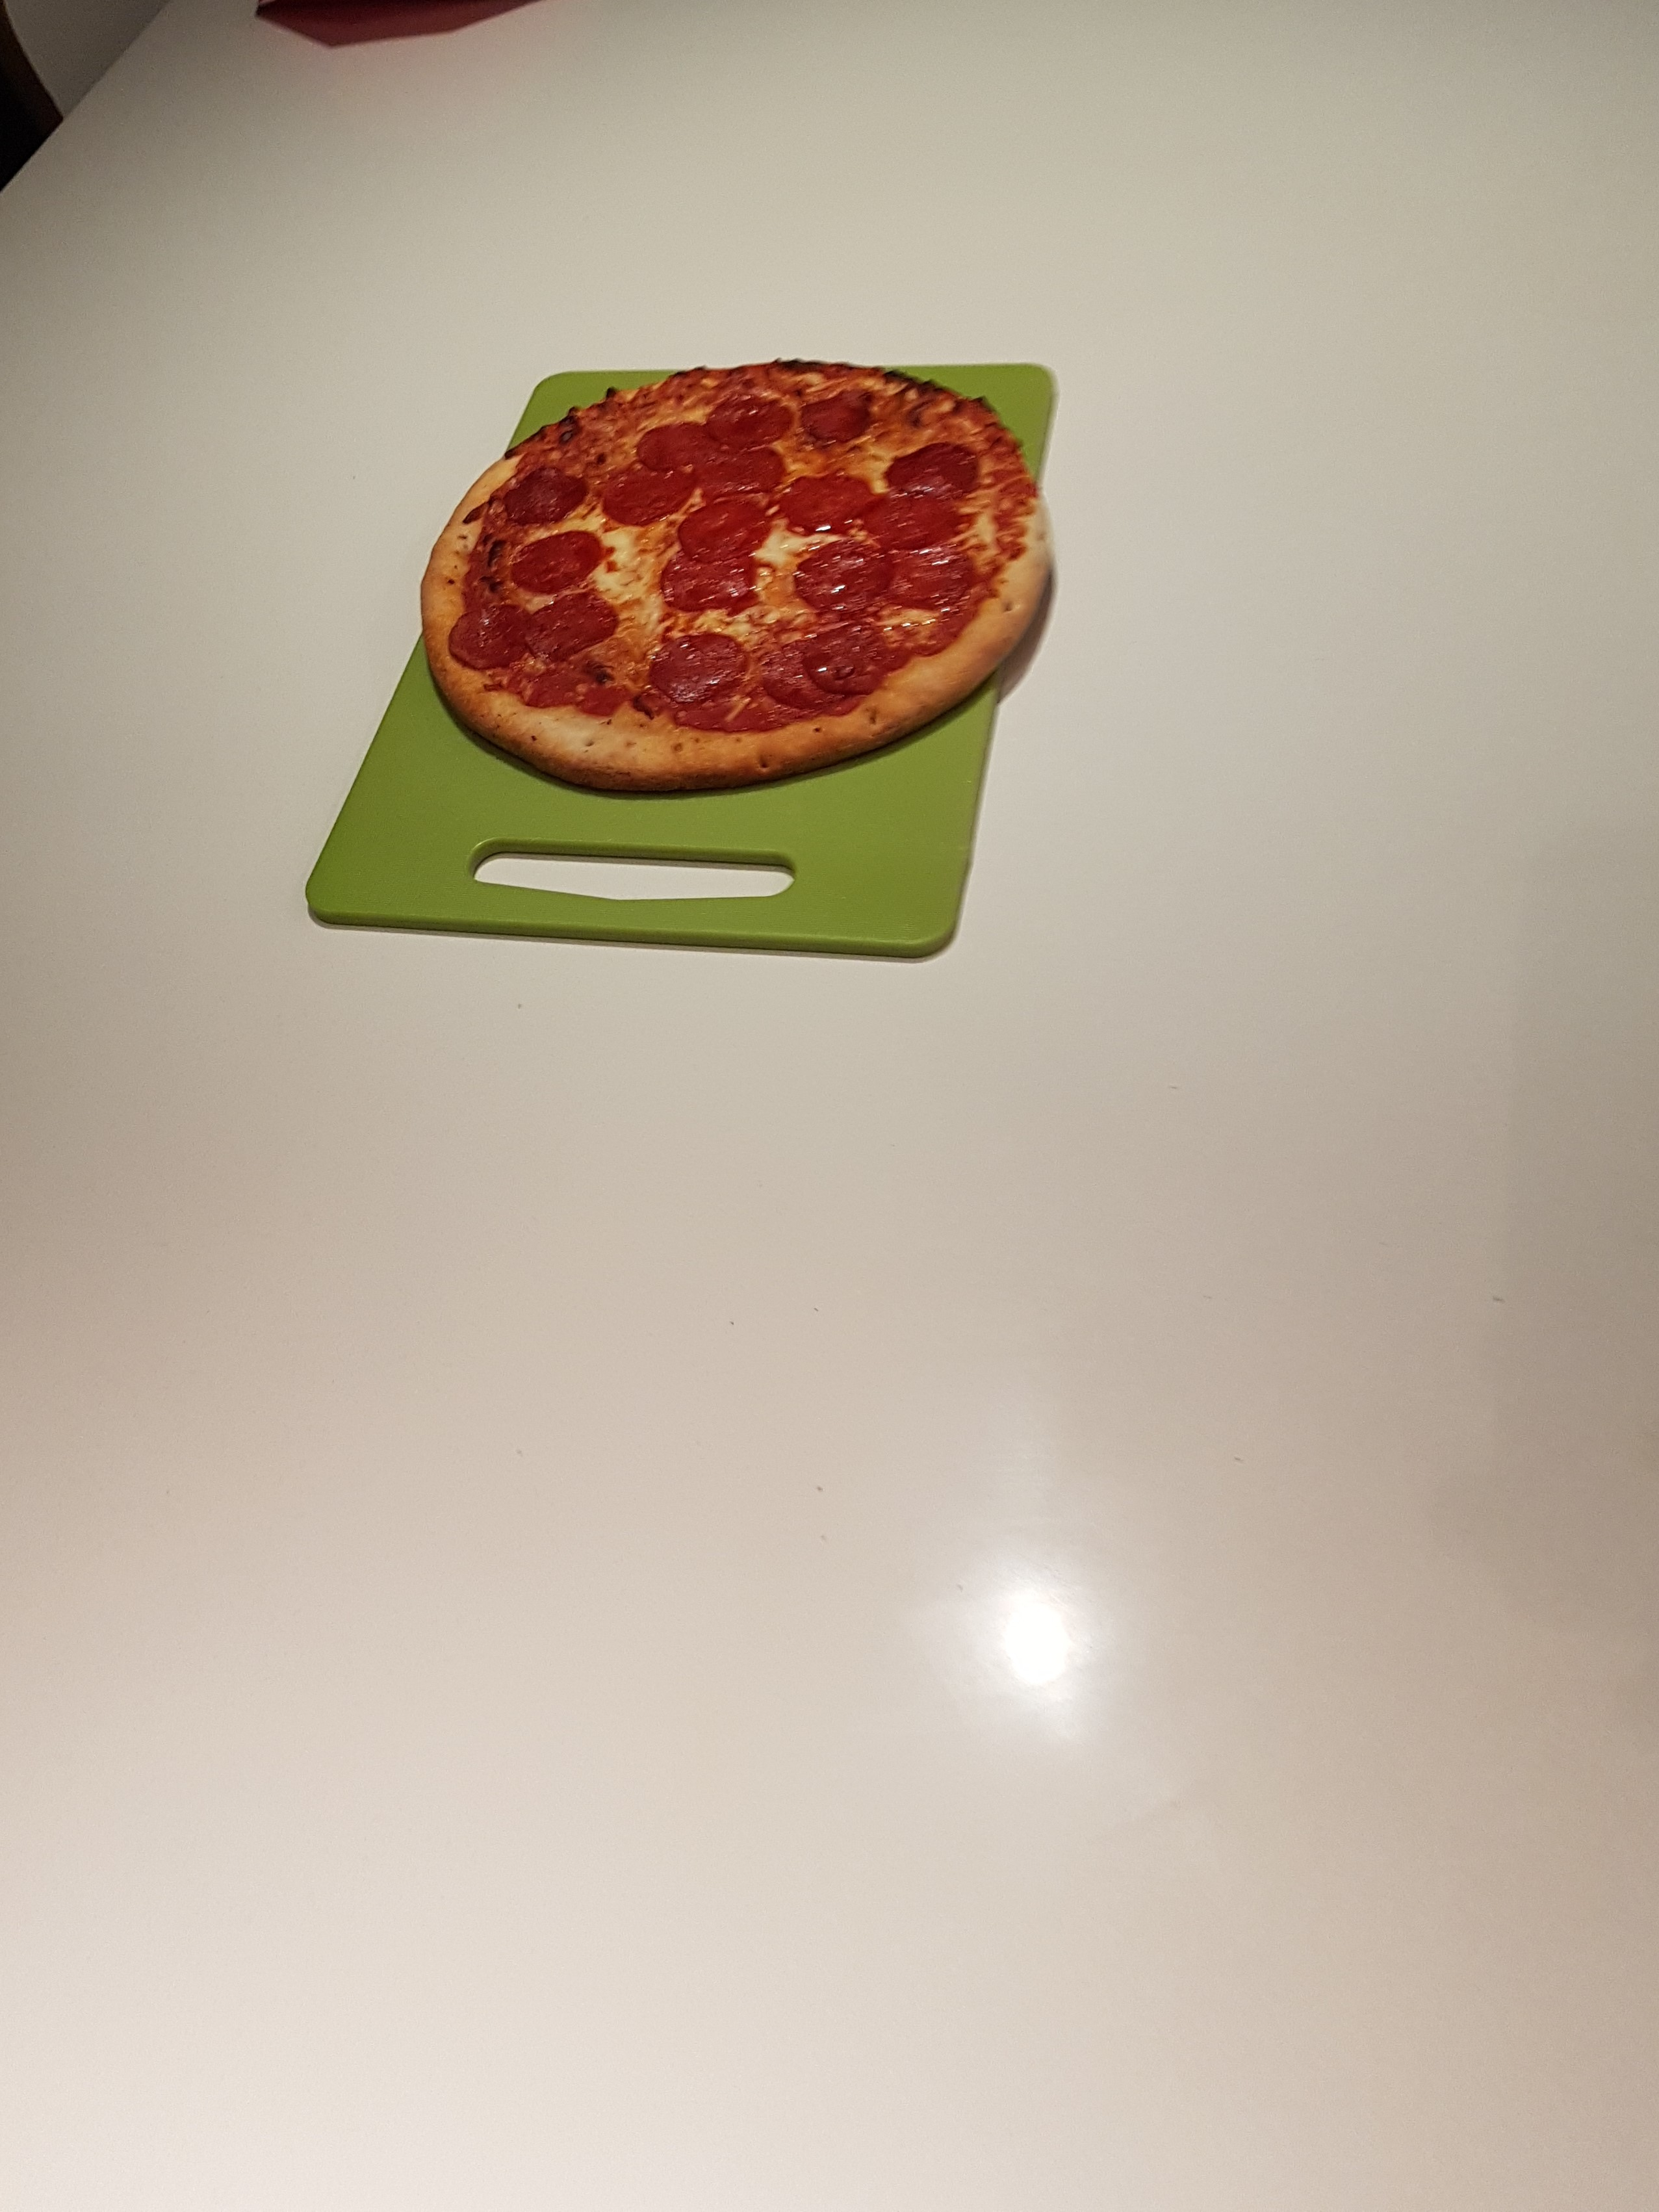
\includegraphics[scale=0.075]{pizza_unclassified}
     \caption{Pizza not classified correctly by the model}
     \label{fig:pizza_unclassified}
\end{figure}

\subsection*{Empirical Analysis}
These poor results are not that surprising.
This is because we have many classes to train for, 101, and no parameter tuning has been carried out on the running of this code.

Figure \ref{fig:pizza_unclassified} was not classified correctly, this is most likely due to the fact that the pizza does not take up much of the image.

